\documentclass[border=8pt]{standalone}
\usepackage{tikz}
\usepackage{amsmath}
\usetikzlibrary{positioning,calc,fit,arrows.meta,backgrounds}
\tikzset{
  lat/.style ={circle, draw=black, fill=white,    minimum size=1.0cm, inner sep=1pt},
  res/.style ={circle, draw=black!55, fill=white, minimum size=0.62cm, inner sep=0pt, font=\small},
  det/.style ={rectangle, rounded corners=3pt, draw=black, fill=blue!7, minimum size=0.95cm, inner sep=3pt},
  obs/.style ={circle, draw=black, fill=black!14,  minimum size=0.95cm, inner sep=1pt},
  inp/.style ={circle, draw=black!55, dashed, fill=white, minimum size=0.7cm, inner sep=1pt, font=\small},
  pl/.style  ={draw=black!50, rounded corners=5pt, inner sep=10pt},
  pll/.style ={font=\footnotesize\itshape, black!55},
  e/.style   ={-{Latex[length=2mm]}, draw=black!75},
  el/.style  ={font=\small, inner sep=1.5pt, fill=white},
}
\begin{document}
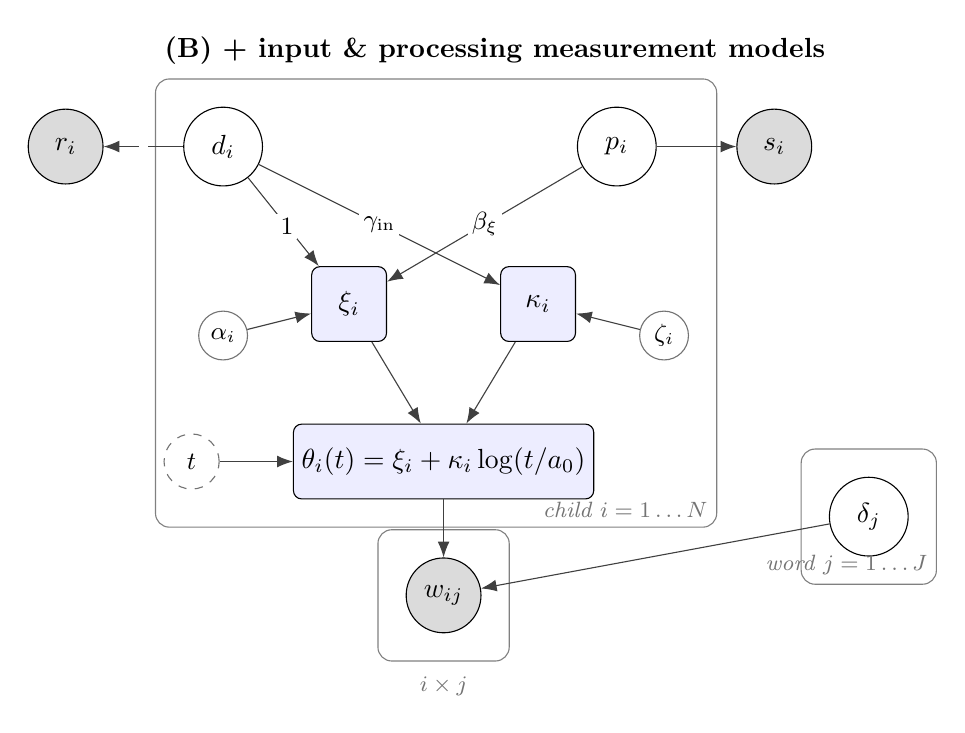
\begin{tikzpicture}
% measurement latents + their observed emissions
\node[lat] (d) at (0,3) {$d_i$};            % input deviation
\node[lat] (p) at (5,3) {$p_i$};            % processing (rt0)
\node[obs] (r) at (-2,3) {$r_i$};           % observed input
\node[obs] (s) at (7,3) {$s_i$};            % observed RT
\draw[e] (d) -- (r) node[el, midway] {};
\draw[e] (p) -- (s);
% structural child traits (deterministic)
\node[det] (xi) at (1.6,1) {$\xi_i$};
\node[det] (ka) at (4.0,1) {$\kappa_i$};
\node[res] (al) at (0.0,0.6) {$\alpha_i$};
\node[res] (ze) at (5.6,0.6) {$\zeta_i$};
\draw[e] (d) -- (xi) node[el, pos=.55] {$1$};
\draw[e] (d) -- (ka) node[el, pos=.5] {$\gamma_{\text{in}}$};
\draw[e] (p) -- (xi) node[el, pos=.5] {$\beta_{\xi}$};
\draw[e] (al) -- (xi);  \draw[e] (ze) -- (ka);
% accumulator core
\node[det] (th) at (2.8,-1.0) {$\theta_i(t)=\xi_i+\kappa_i\log(t/a_0)$};
\node[inp] (t) at (-0.4,-1.0) {$t$};
\node[obs] (w) at (2.8,-2.7) {$w_{ij}$};
\node[lat] (de) at (8.2,-1.7) {$\delta_j$};
\draw[e] (xi) -- (th); \draw[e] (ka) -- (th); \draw[e] (t) -- (th);
\draw[e] (th) -- (w);  \draw[e] (de) -- (w);
% plates
\begin{scope}[on background layer]
\node[pl, fit=(d)(p)(xi)(ka)(al)(ze)(th)] (childpl) {};
\node[pl, fit=(de)] (wordpl) {};
\node[pl, fit=(w)] (obspl) {};
\end{scope}
\node[pll, anchor=south east] at (childpl.south east) {child $i=1\ldots N$};
\node[pll, anchor=south east] at (wordpl.south east) {word $j=1\ldots J$};
\node[pll, anchor=north] at ([yshift=-2pt]obspl.south) {$i\times j$};
\node[font=\bfseries, anchor=west] at ([yshift=10pt]childpl.north west) {(B) + input \& processing measurement models};
\end{tikzpicture}
\end{document}
